\begin{frame} \frametitle{US pulse and Trapezoidal acoustic waveforms are used.}
  \begin{figure}
    \centering
    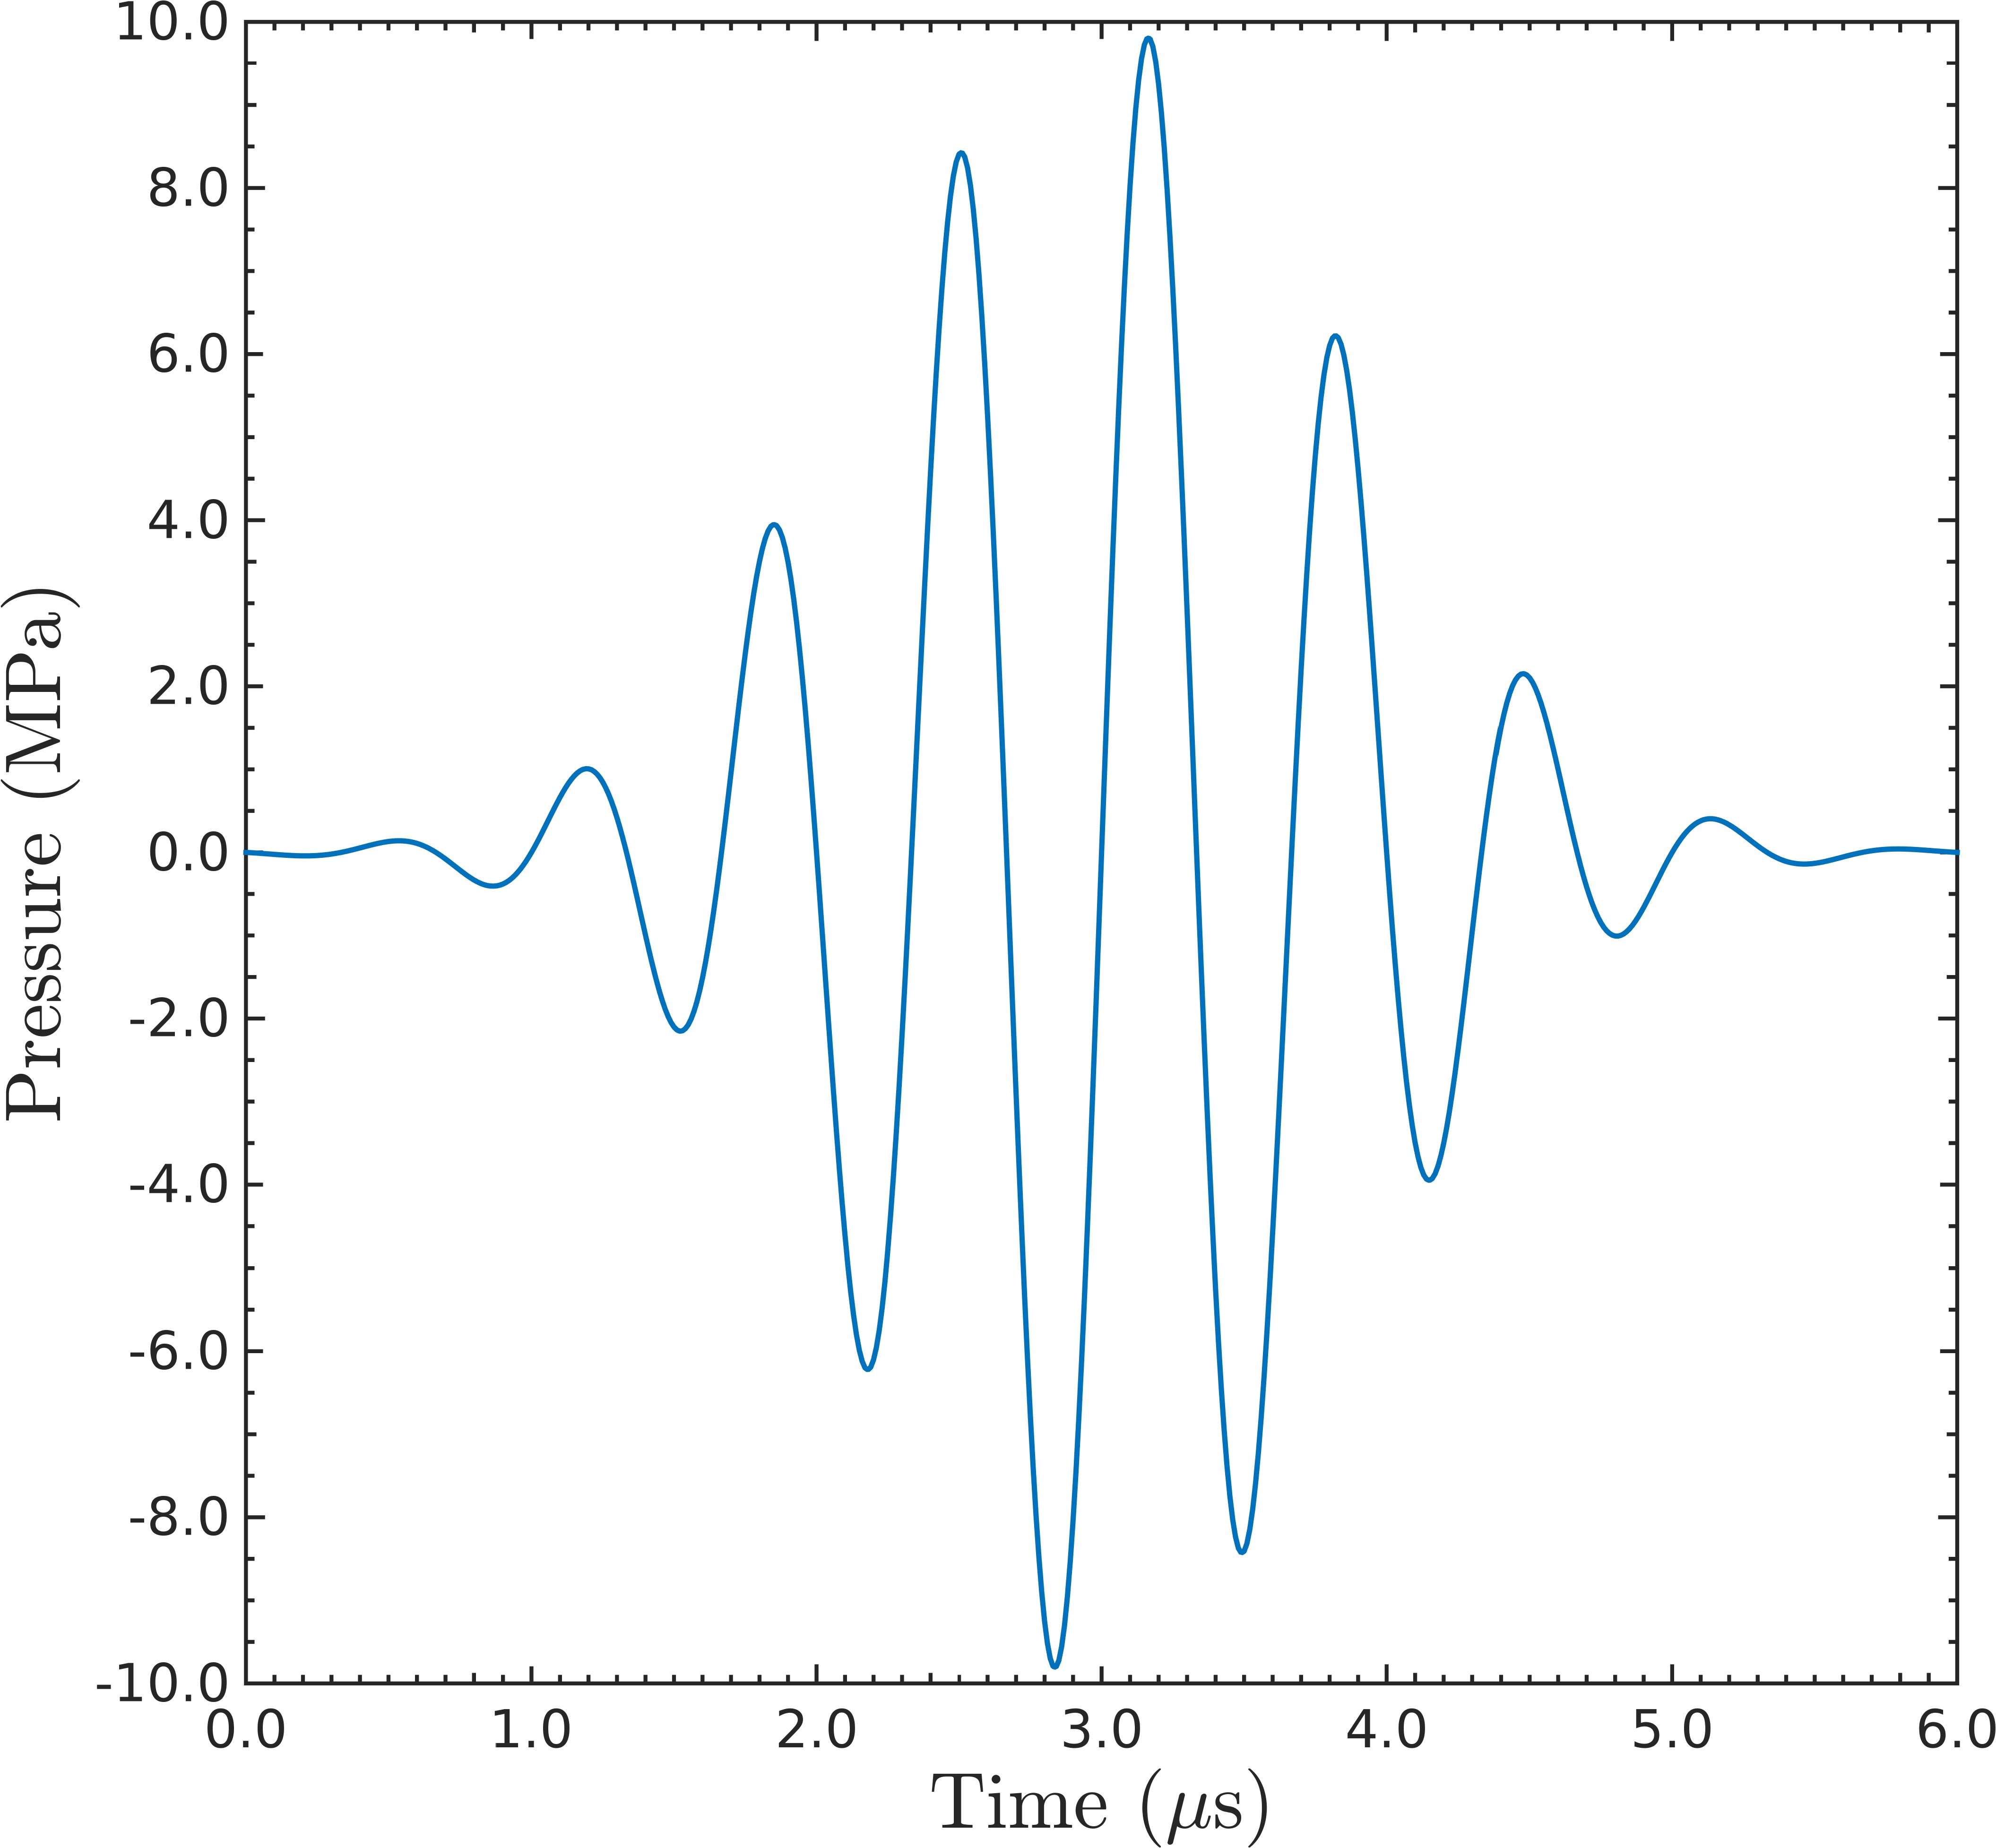
\includegraphics[height=0.4\textheight]{../figs/lung_figs/p0_vs_t_us}\hfill%
    \visible<2->{
    \def\svgwidth{0.25\textwidth}
      {\footnotesize
        \import{../figs/lung_figs/}{wave_logic_schematic2.pdf_tex}%
      }
    }
    \hfill%
    \visible<3->{
    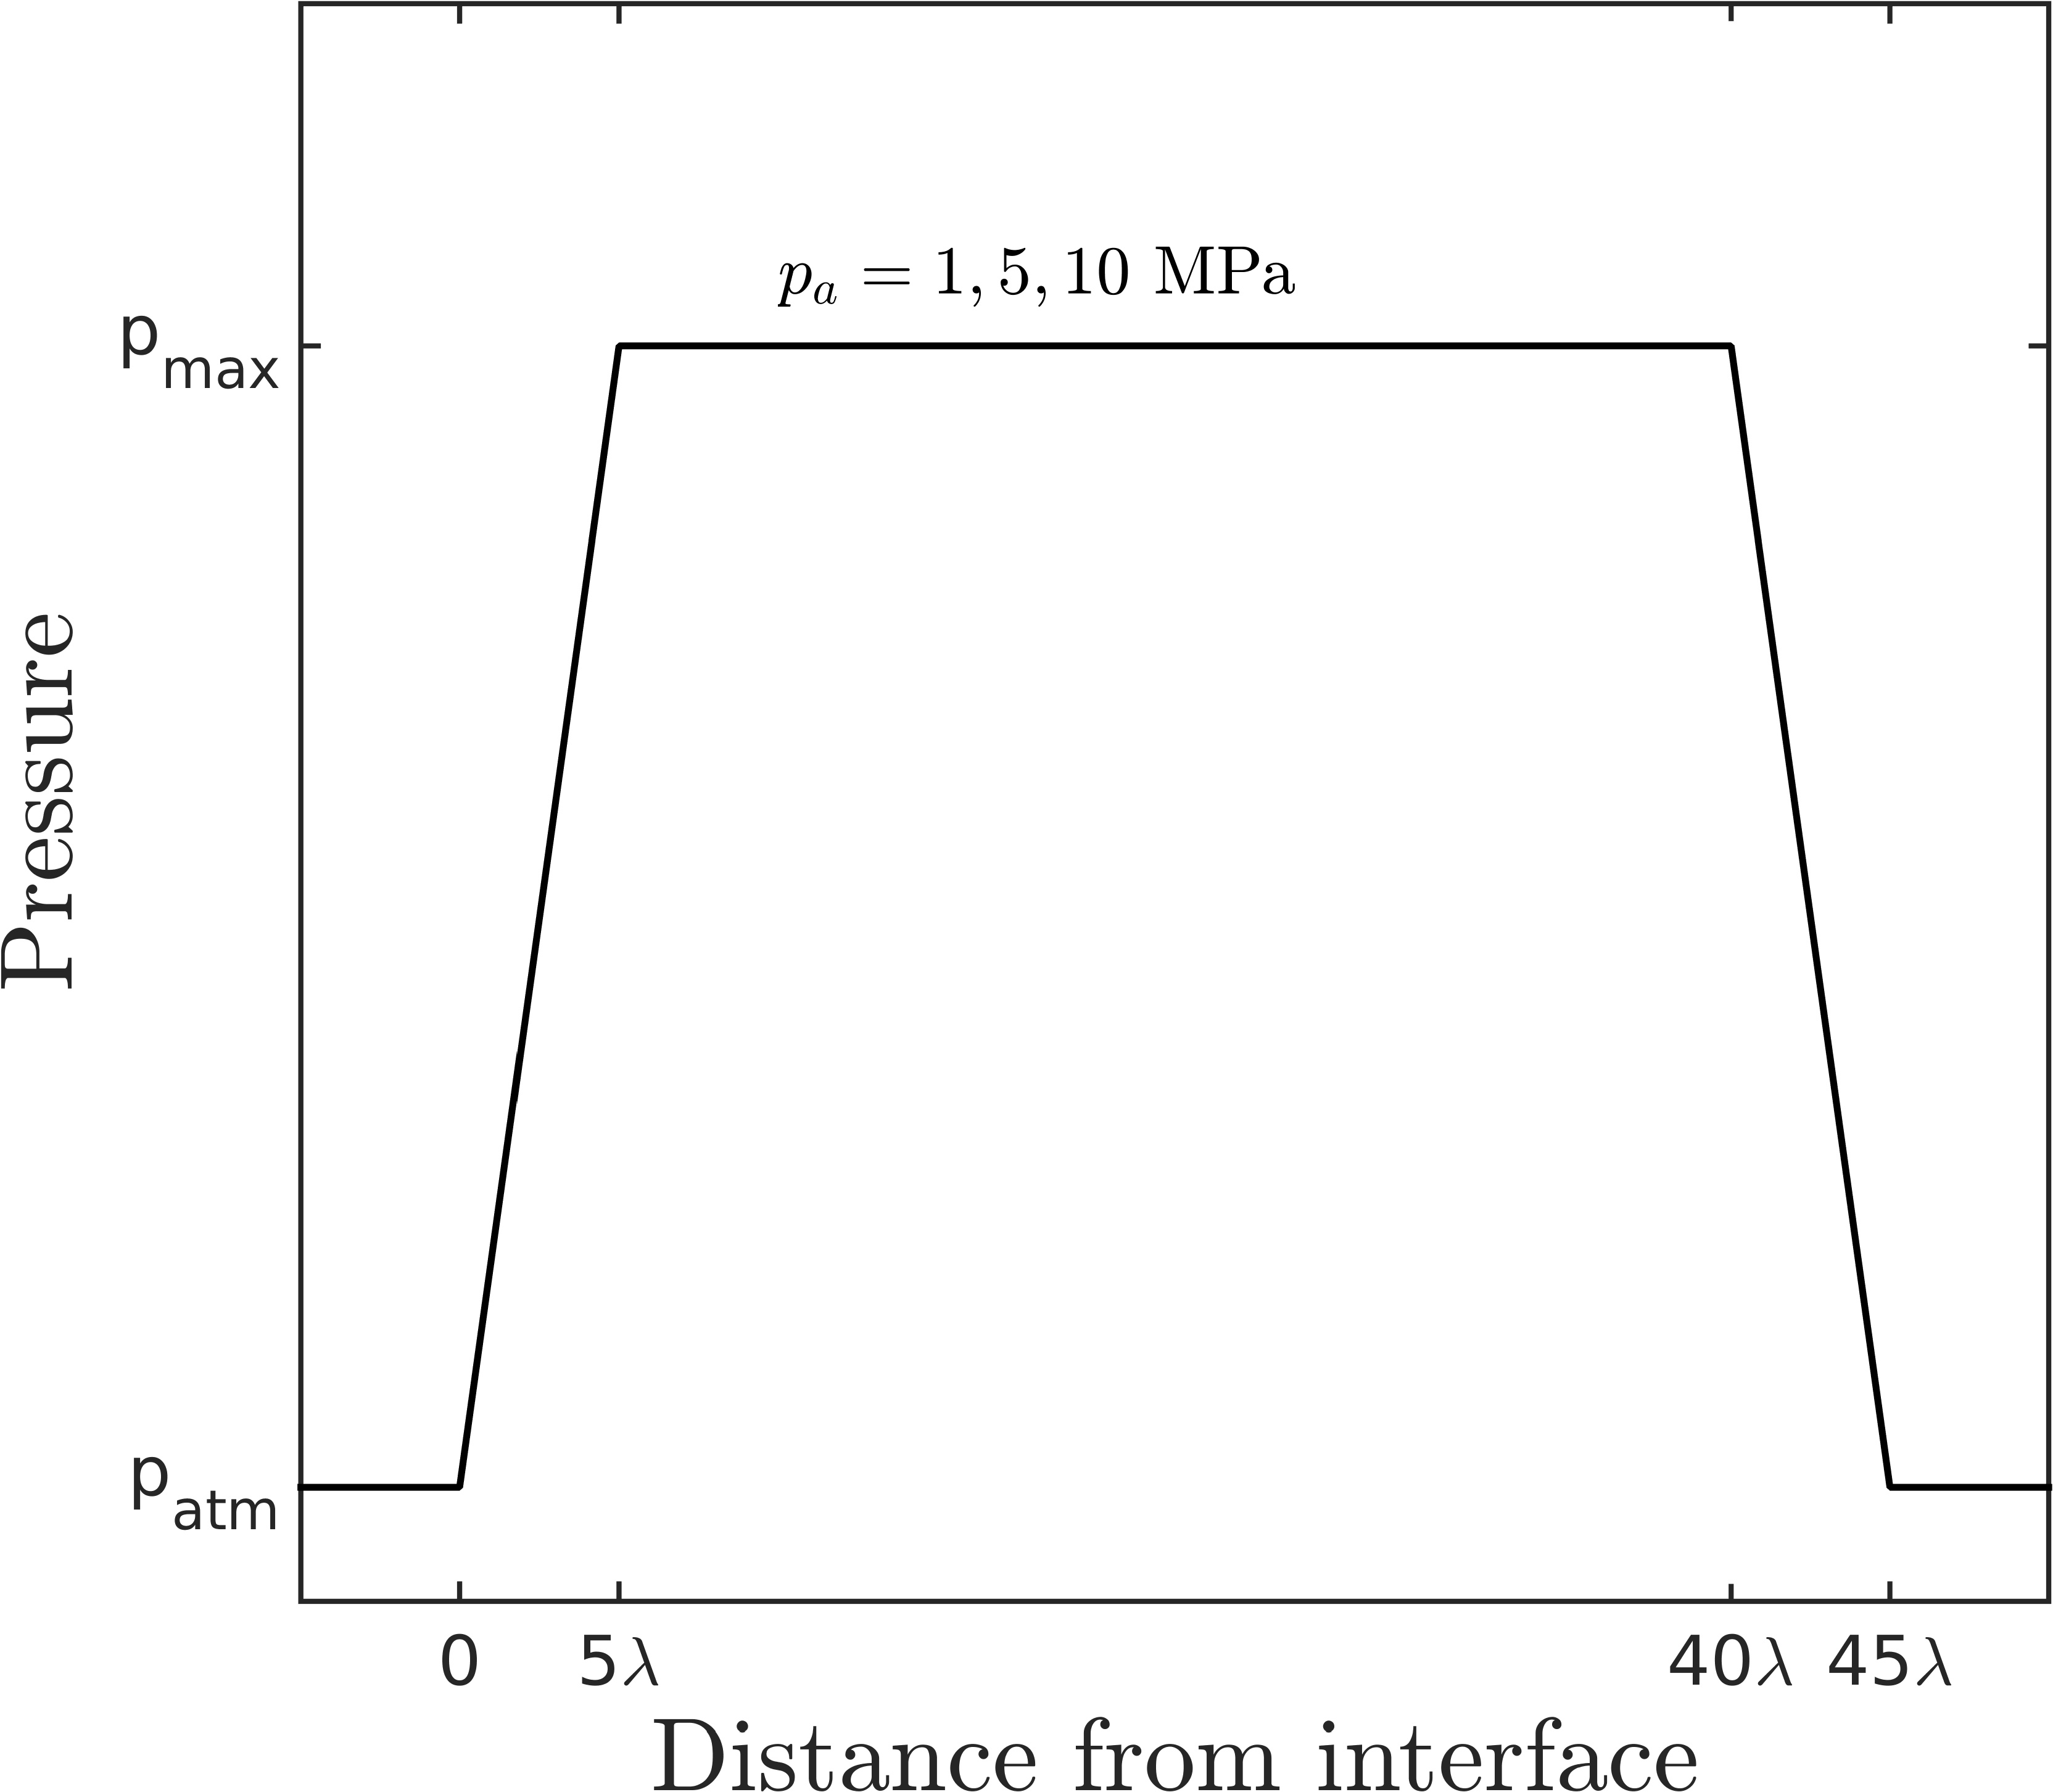
\includegraphics[height=0.4\textheight]{../figs/lung_figs/p0_vs_y}%
    }
  \end{figure}
  \visible<3->{
    \begin{itemize}
    \item The trapezoidal waves is simple for understanding physics and analysis, but able to capture feature of US pulse.
    \item Pulse waveforms are used to check relevance to DUS.
    \end{itemize}
  }
  \note{
    \begin{enumerate}
    \item To simplify the wave, we can fouirer decompose a DUS pulse and think of it as a sum of sin waves.
    \item Each sin is a sum of two half-sines, which can be approximated as trapezoidal waves.
    \item These waveforms are used because they can be readily analyzed, but they are designed to capture features of DUS.
    \item Ratio of pulse length to alveolar length and pressure gradients are designed to reflect clinical DUS.
    \item For example, the pulses used interact with the interface for about $3$ microseconds, which is roughly half the length of a DUS pulse.
    \item 1, 5, and 10 MPa waves considered, but results today are from 5, 10. 1 is too slow for computational reasons. 15 is running.
    \end{enumerate}
  }
\end{frame}
%%% Local Variables:
%%% mode: latex
%%% TeX-master: "../main"
%%% End:
